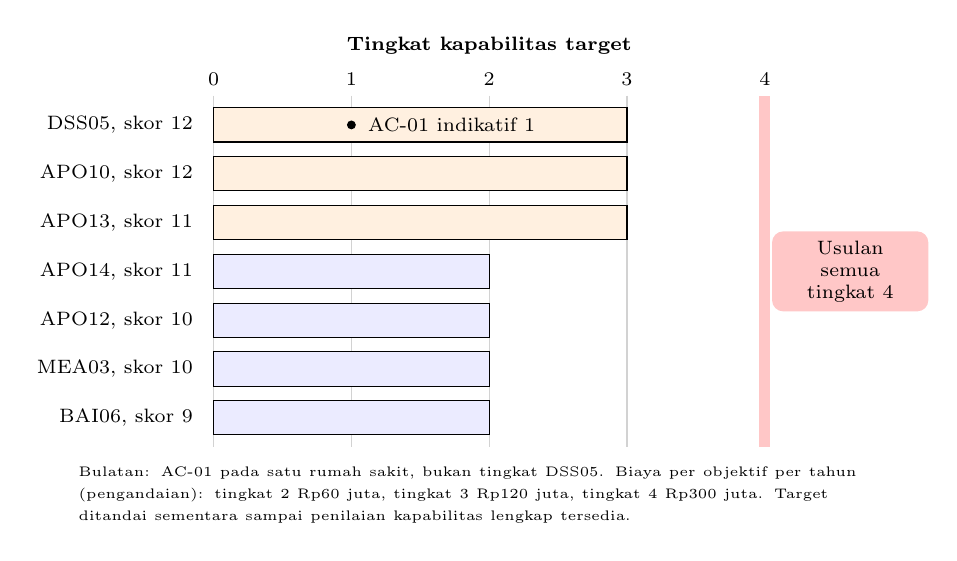
\begin{tikzpicture}[
  font=\scriptsize,
  x=1.75cm,
  y=0.62cm,
  batang3/.style={draw, fill=orange!12},
  batang2/.style={draw, fill=blue!8}]
  \foreach \tingkat in {0,1,2,3} {
    \draw[gray!35] (\tingkat,0.6) -- (\tingkat,-6.6);
    \node[above] at (\tingkat,0.6) {\tingkat};
  }
  \fill[red!22] (3.96,0.6) rectangle (4.04,-6.6);
  \node[above] at (4,0.6) {4};
  \node[fill=red!22, align=center, rounded corners, text width=1.75cm] at (4.62,-3)
    {Usulan\\semua\\tingkat 4};
  \node[above, font=\scriptsize\bfseries] at (2,1.25) {Tingkat kapabilitas target};
  \node[anchor=east] at (-0.08,0) {DSS05, skor 12};
  \node[anchor=east] at (-0.08,-1) {APO10, skor 12};
  \node[anchor=east] at (-0.08,-2) {APO13, skor 11};
  \node[anchor=east] at (-0.08,-3) {APO14, skor 11};
  \node[anchor=east] at (-0.08,-4) {APO12, skor 10};
  \node[anchor=east] at (-0.08,-5) {MEA03, skor 10};
  \node[anchor=east] at (-0.08,-6) {BAI06, skor 9};
  \draw[batang3] (0,-0.35) rectangle (3,0.35);
  \draw[batang3] (0,-1.35) rectangle (3,-0.65);
  \draw[batang3] (0,-2.35) rectangle (3,-1.65);
  \draw[batang2] (0,-3.35) rectangle (2,-2.65);
  \draw[batang2] (0,-4.35) rectangle (2,-3.65);
  \draw[batang2] (0,-5.35) rectangle (2,-4.65);
  \draw[batang2] (0,-6.35) rectangle (2,-5.65);
  \fill (1,0) circle (1.6pt);
  \node[anchor=west] at (1.05,0) {AC-01 indikatif 1};
  \node[anchor=north west, align=left, text width=10cm] at (-1.05,-6.8)
    {{\tiny\mdseries Bulatan: AC-01 pada satu rumah sakit, bukan tingkat DSS05. Biaya per objektif
    per tahun (pengandaian): tingkat 2 Rp60 juta, tingkat 3 Rp120 juta, tingkat 4 Rp300 juta.
    Target ditandai sementara sampai penilaian kapabilitas lengkap tersedia.}};
\end{tikzpicture}
